\begin{figure}[htbp]
  \centering
  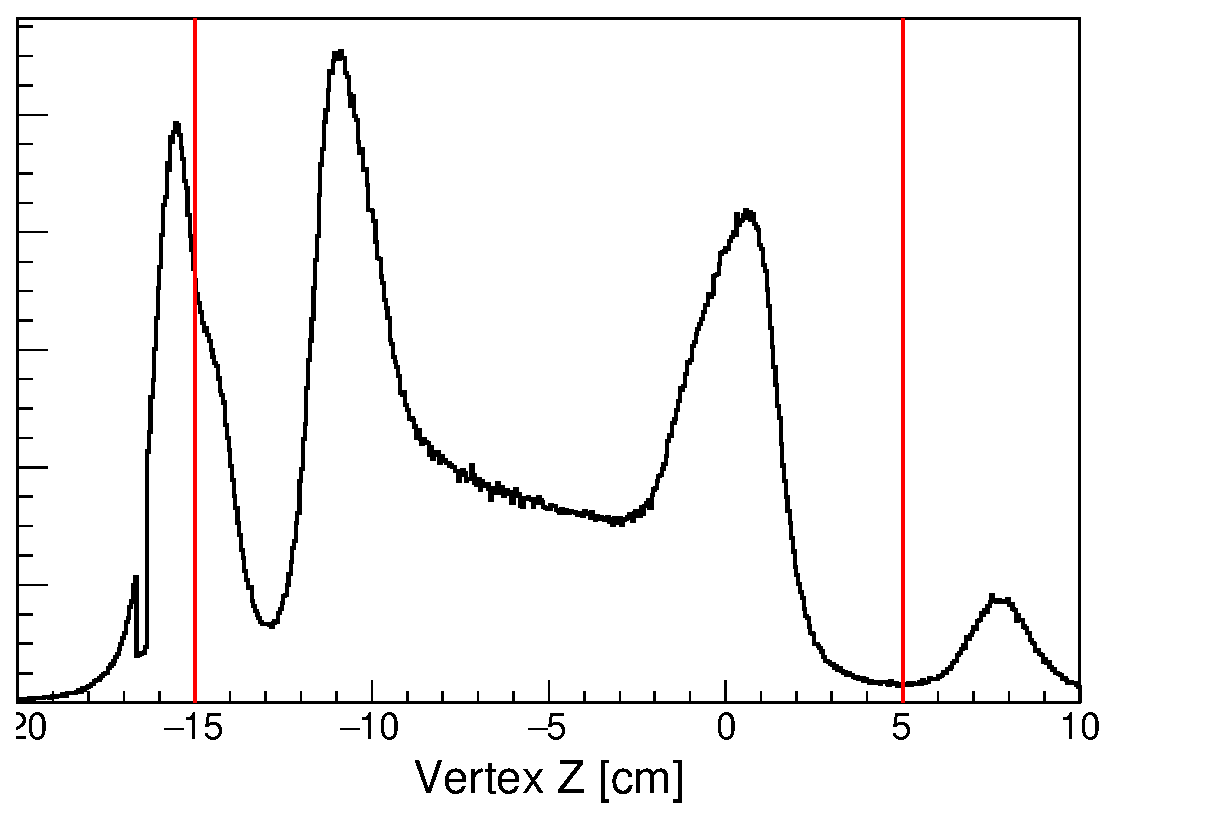
\includegraphics[width=8cm]{../pic/Run78/CDS/vertex.eps}
  \caption{
    Recionstructed vertex point distrivution by the BPC and CDC.
    Right figure shows about $xy$ plane.
    Up figure and down figure of lift side was shows $yz$ plane and $xz$ plane, respectively.
  }
  \label{fig:vertex}
\end{figure}

\subsection{Vertex reconstruction}
The reaction vertex point was calculated from the beam track by the BPC and the CDC tracks.
First, the CDC track which gives the distance of the closest approach (DCA) was searched and the reaction vertex point was defined by closest point of the beam track.
Fig\ref{fig:vertex} shows reconstructed reaction vertex images.
We used the target chamber with $6.8cm$ diameter PET whose image was clearly shown in $xy$ plane figure.
$D_2$ target transfer pipes placed parallel to the floor was shown at $z=8cm$ in light side figures,
also DEF counter installed just upstream of the target chamber was seen at about $z=-15cm$.
%% todo target-imageにFiducialの追加

For evaluation of the vertex resolution, some projected histograms was made.
The $xy$ vertex resolution was evaluated at some range of z axis and target center of y as left figure of Fig\ref{fig:vertex_pro}.
The $xy$ vertex resolution was evaluated about $1.4mm$.
The $z$ vertex resolution was evaluated by the DEF counter using z axis projection histogram at $r<3cm$.
The $z$ vertex resolution was evaluated about $7.0mm$.

\begin{figure}[htbp]
  \centering
  \begin{tabular}{cc}
    \begin{minipage}{0.5\hsize}
      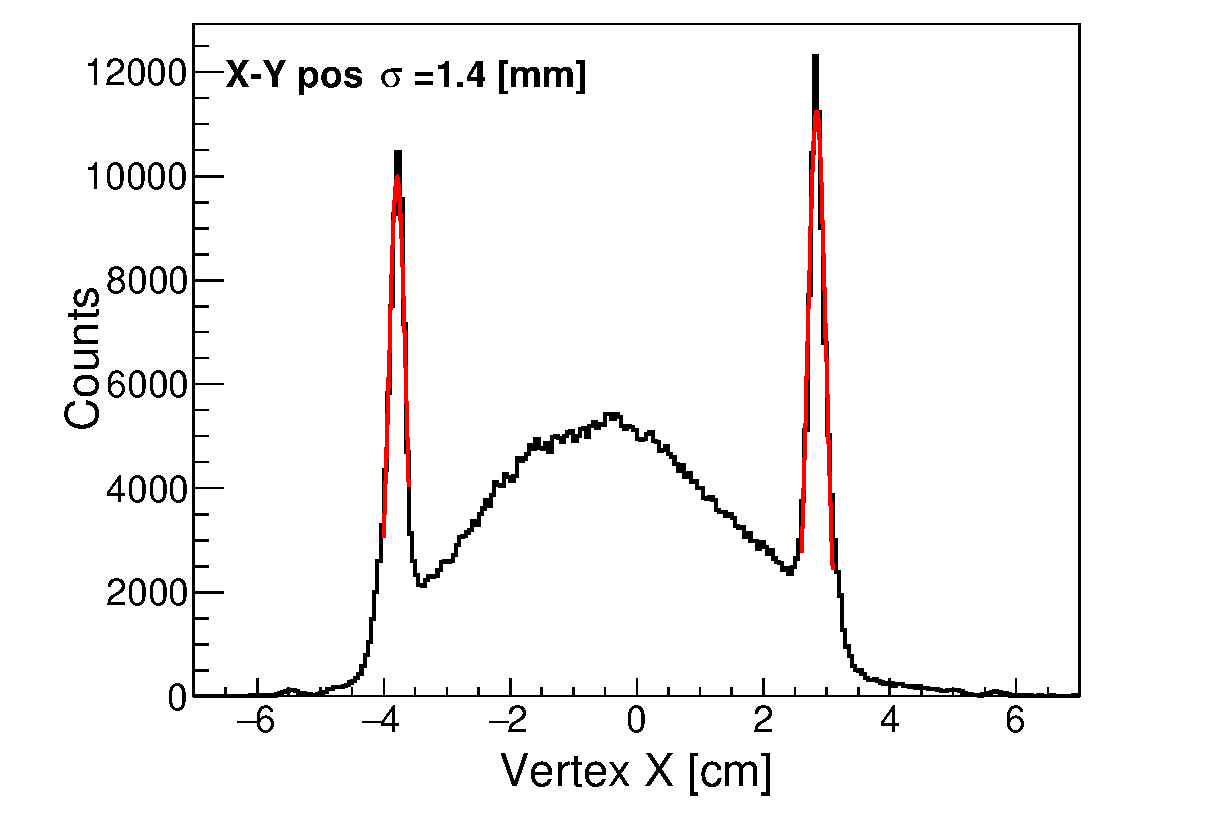
\includegraphics[width=6cm]{../pic/Run78/CDS/vertex_x.eps}
    \end{minipage}

    \begin{minipage}{0.5\hsize}
      \includegraphics[width=6cm]{../pic/Run78/CDS/vertex_z.eps}
    \end{minipage}
  \end{tabular}
  \caption{
    Left figure shows x axis projection at $y=0cm$ and $z>-12.5cm$ to evaluate $xy$ vertex resolution.
    Right figure shows z axis projection at $x^2+y^2<3cm$ to evaluate $z$ vertex resoution.
  }
  \label{fig:vertex_pro}
\end{figure}
